 \section{System model and problem}
\label{sec:Problem description}
In this section, we first introduce  basic concepts on virtual network embedding, then present our survivable virtual network embedding problem.


\subsection{Virtual network embedding}

\note{Pay attention to making the presentation concise without repetition.}

We represent a \textbf{virtual network} (VN) as an undirected graph $G (V,E)$ where $V$ and  $E$ are the sets of virtual nodes and virtual links, respectively. Each virtual link $e_{ij}$ has a bandwidth demand $d_{ij}$. Each virtual node  $v_i$ has \rev{a demand $d_i$ for the computation capacity.}  The virtual function required to be executed on \rev{the virtual node $v_i$ is denoted as $f(i)$.} Fig.\ref{fig:VNQSNVNE}(a) shows an example  with virtual node set $V=\{v_1,v_2,v_3,v_4\}$ and virtual edge set $E= \{e_{12},e_{13},e_{14},e_{23}\}$. The virtual functions required to be executed on these virtual nodes are  $f(1)=f_1$, $f(2)=f_2$, $f(3)=f_3$, $f(4)=f_4$, respectively.
%\begin{figure}
%\centering
%\begin{minipage}[t]{0.45\linewidth}
%% Requires \usepackage{graphicx}
%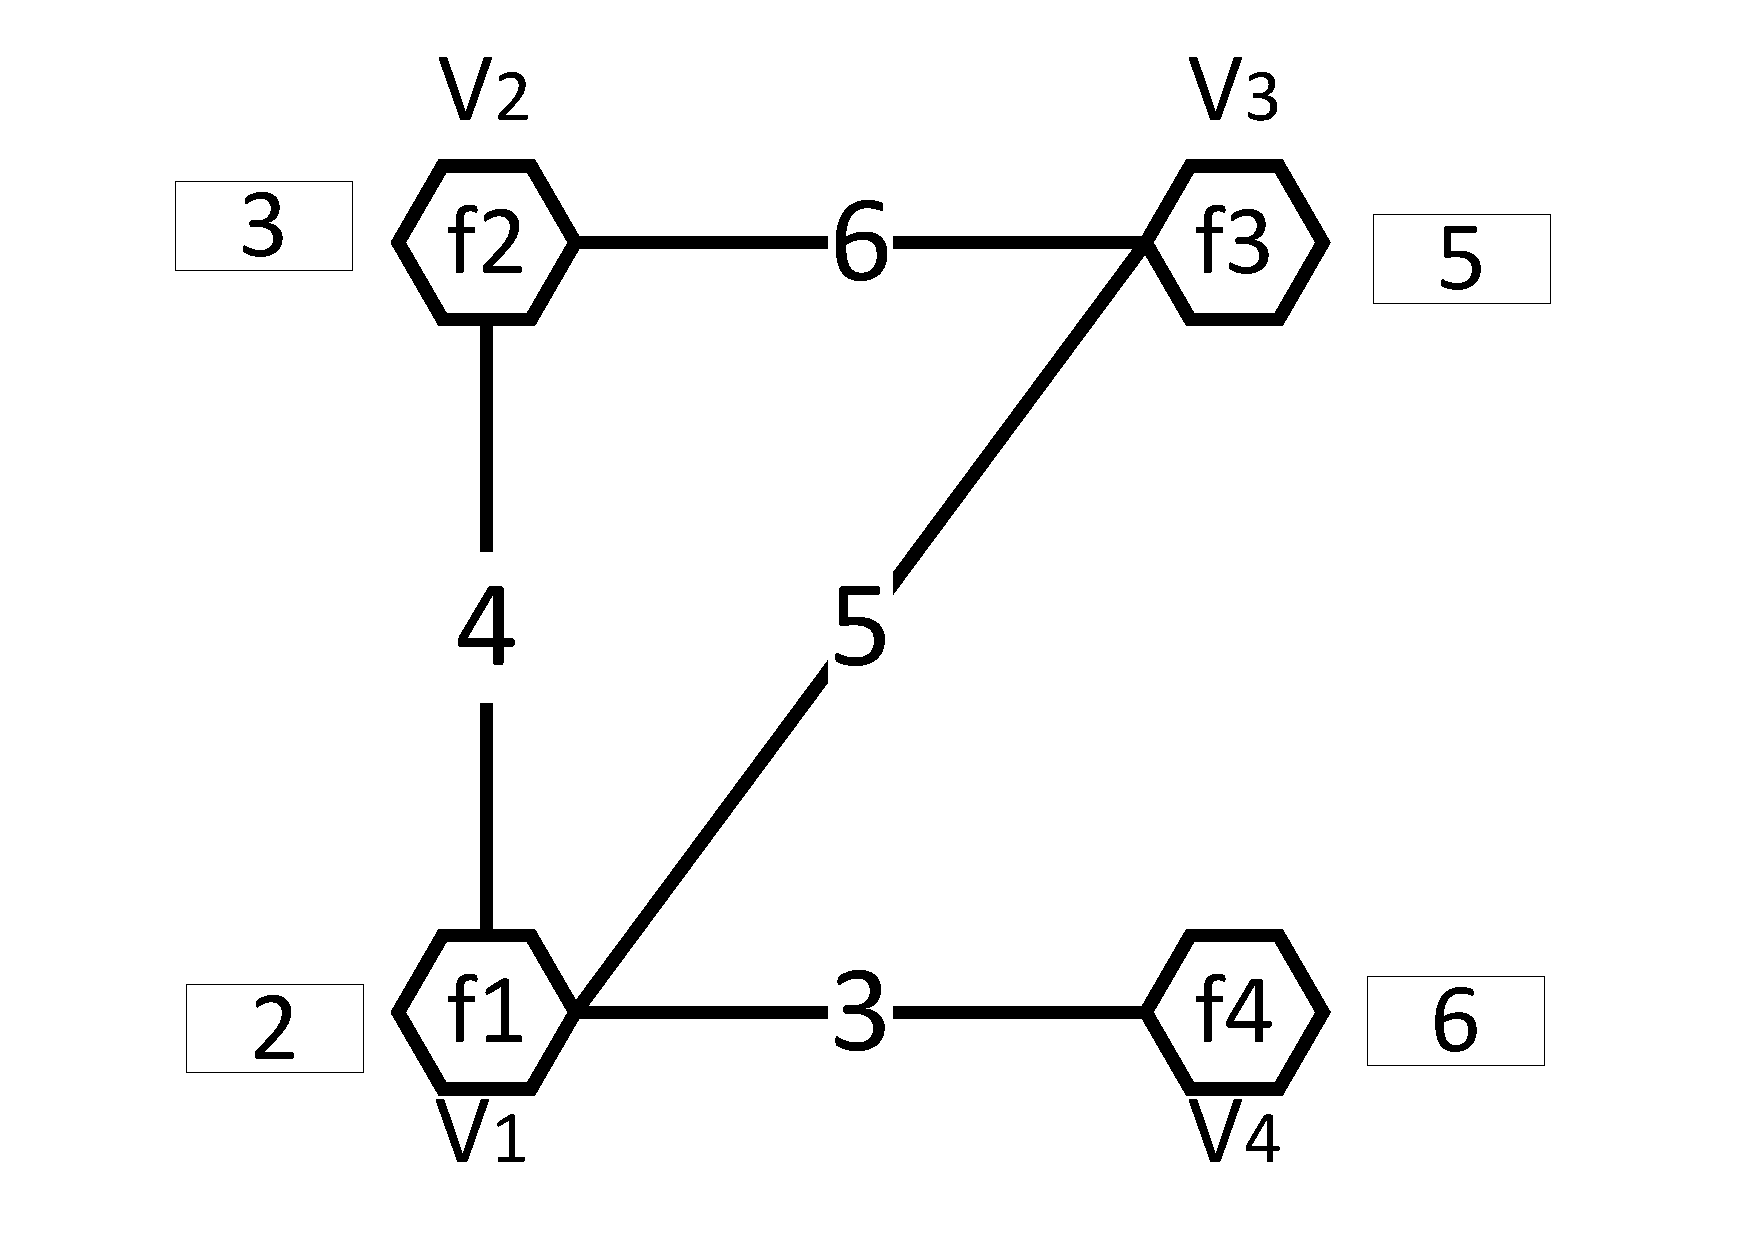
\includegraphics[width=1.3in]{Fig/VNQ}\\
%\caption{Virtual Network Request $G(V,E)$, $V=\{v_1,v_2,v_3,v_4\}$, $E=\{e_{12},e_{23},e_{13},e_{14}\}$,  $f^V=\{f_1,f_2,f_3,f_4\}$, $d_i=\{2,3,5,6\}$, $d_{ij}=\{4,5,3,6\}.$}\label{fig:VNQ}
%\end{minipage}
%\hfill
%\begin{minipage}[t]{0.45\linewidth}
%% Requires \usepackage{graphicx}
%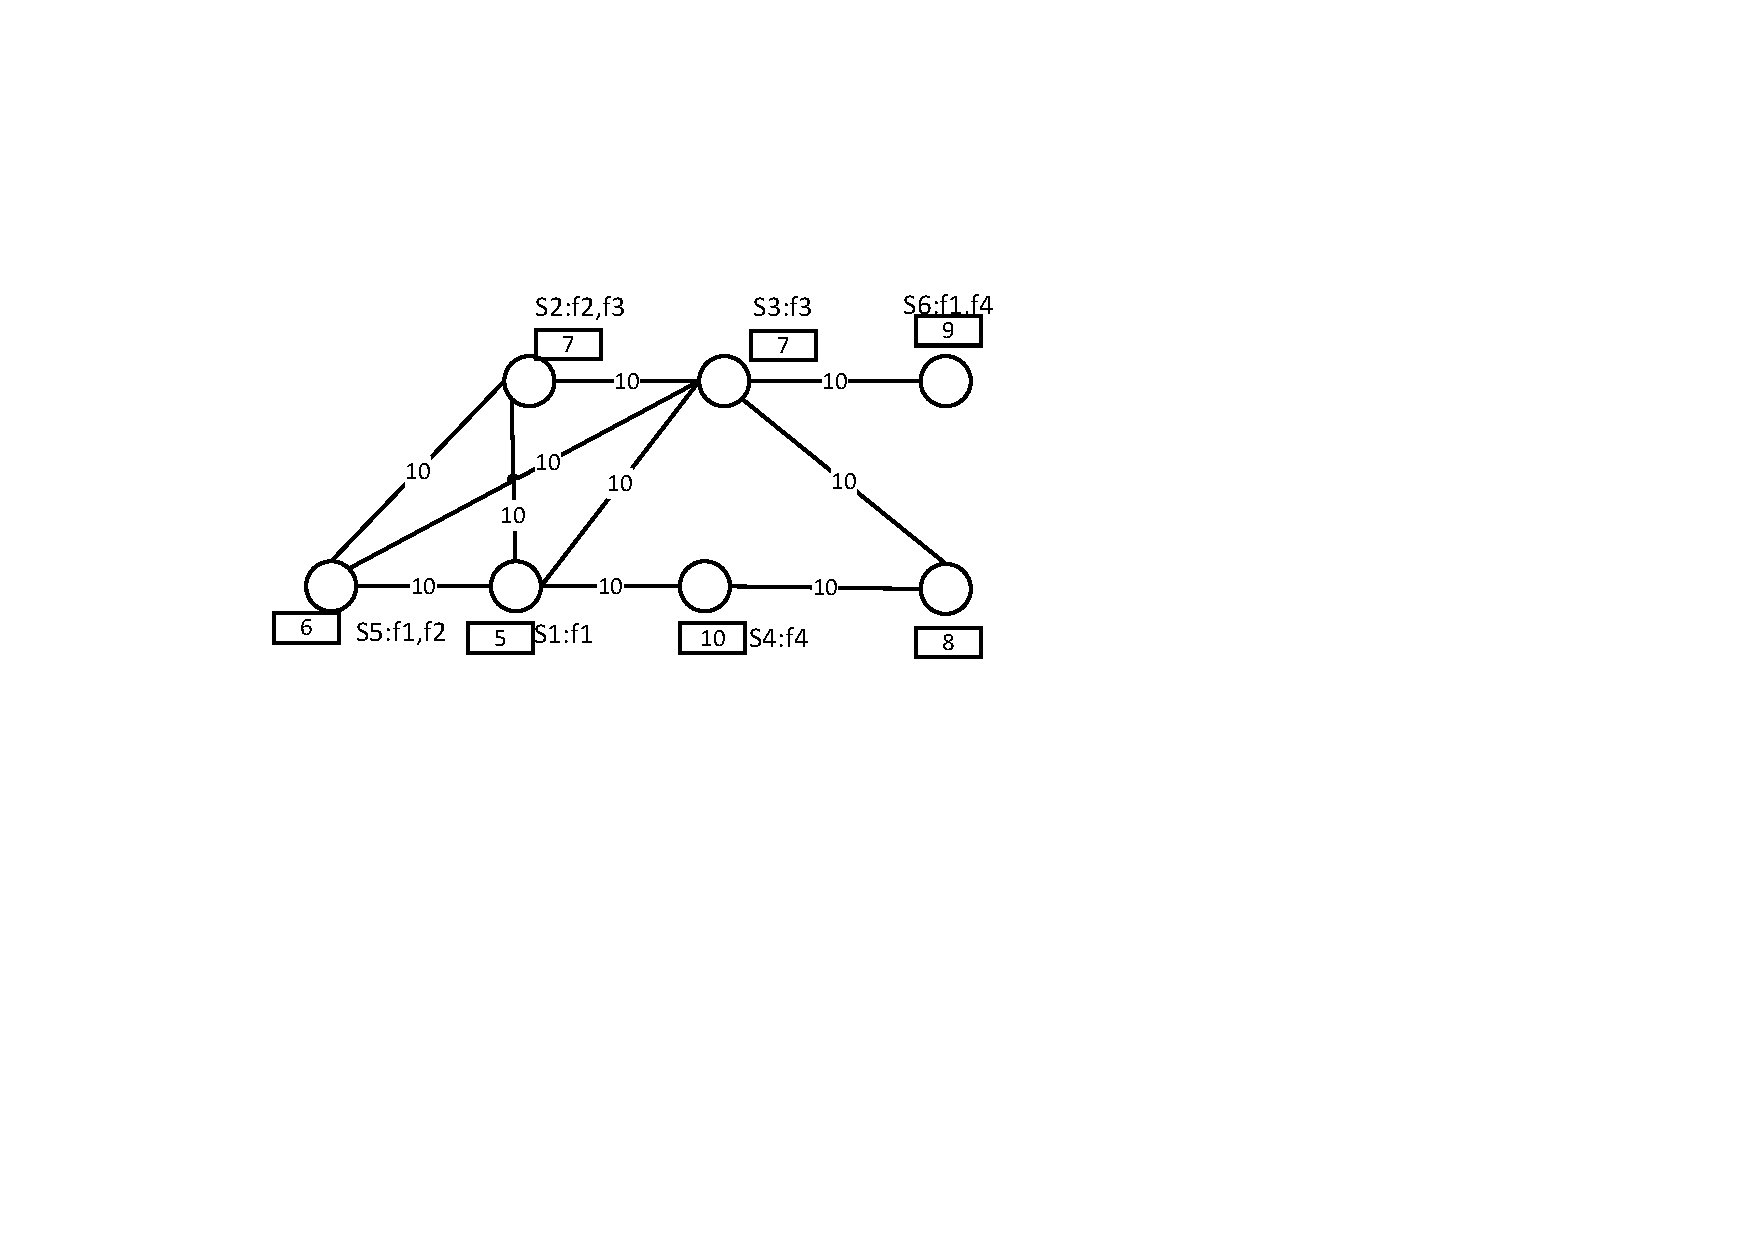
\includegraphics[width=1.8in]{Fig/SN}\\
%\caption{Physical Network $G^S(V^S,E^S), V^S=\{s_1,s_2,s_3,s_4,s_5,s_6,s_7\}, E^S=\{l_{12},l_{13},l_{14},l_{15},l_{23},l_{25},l_{35},l_{36},l_{37},l_{47}\}, F^S=\{\{f_1\},\{f_2,f_3\},\{f_3\},\{f_4\},\{f_1,f_2\},\{f_1,f_4\},\{f_2,f_3\}\}, c_i=\{5,7,7,10,6,9,8\}, %b_{ij}=\{10,10,10,10,10,10,10,10,10,10\}$}\label{fig:SN}
%\end{minipage}
%\end{figure}

\begin{figure*}
\centering
% Requires \usepackage{graphicx}
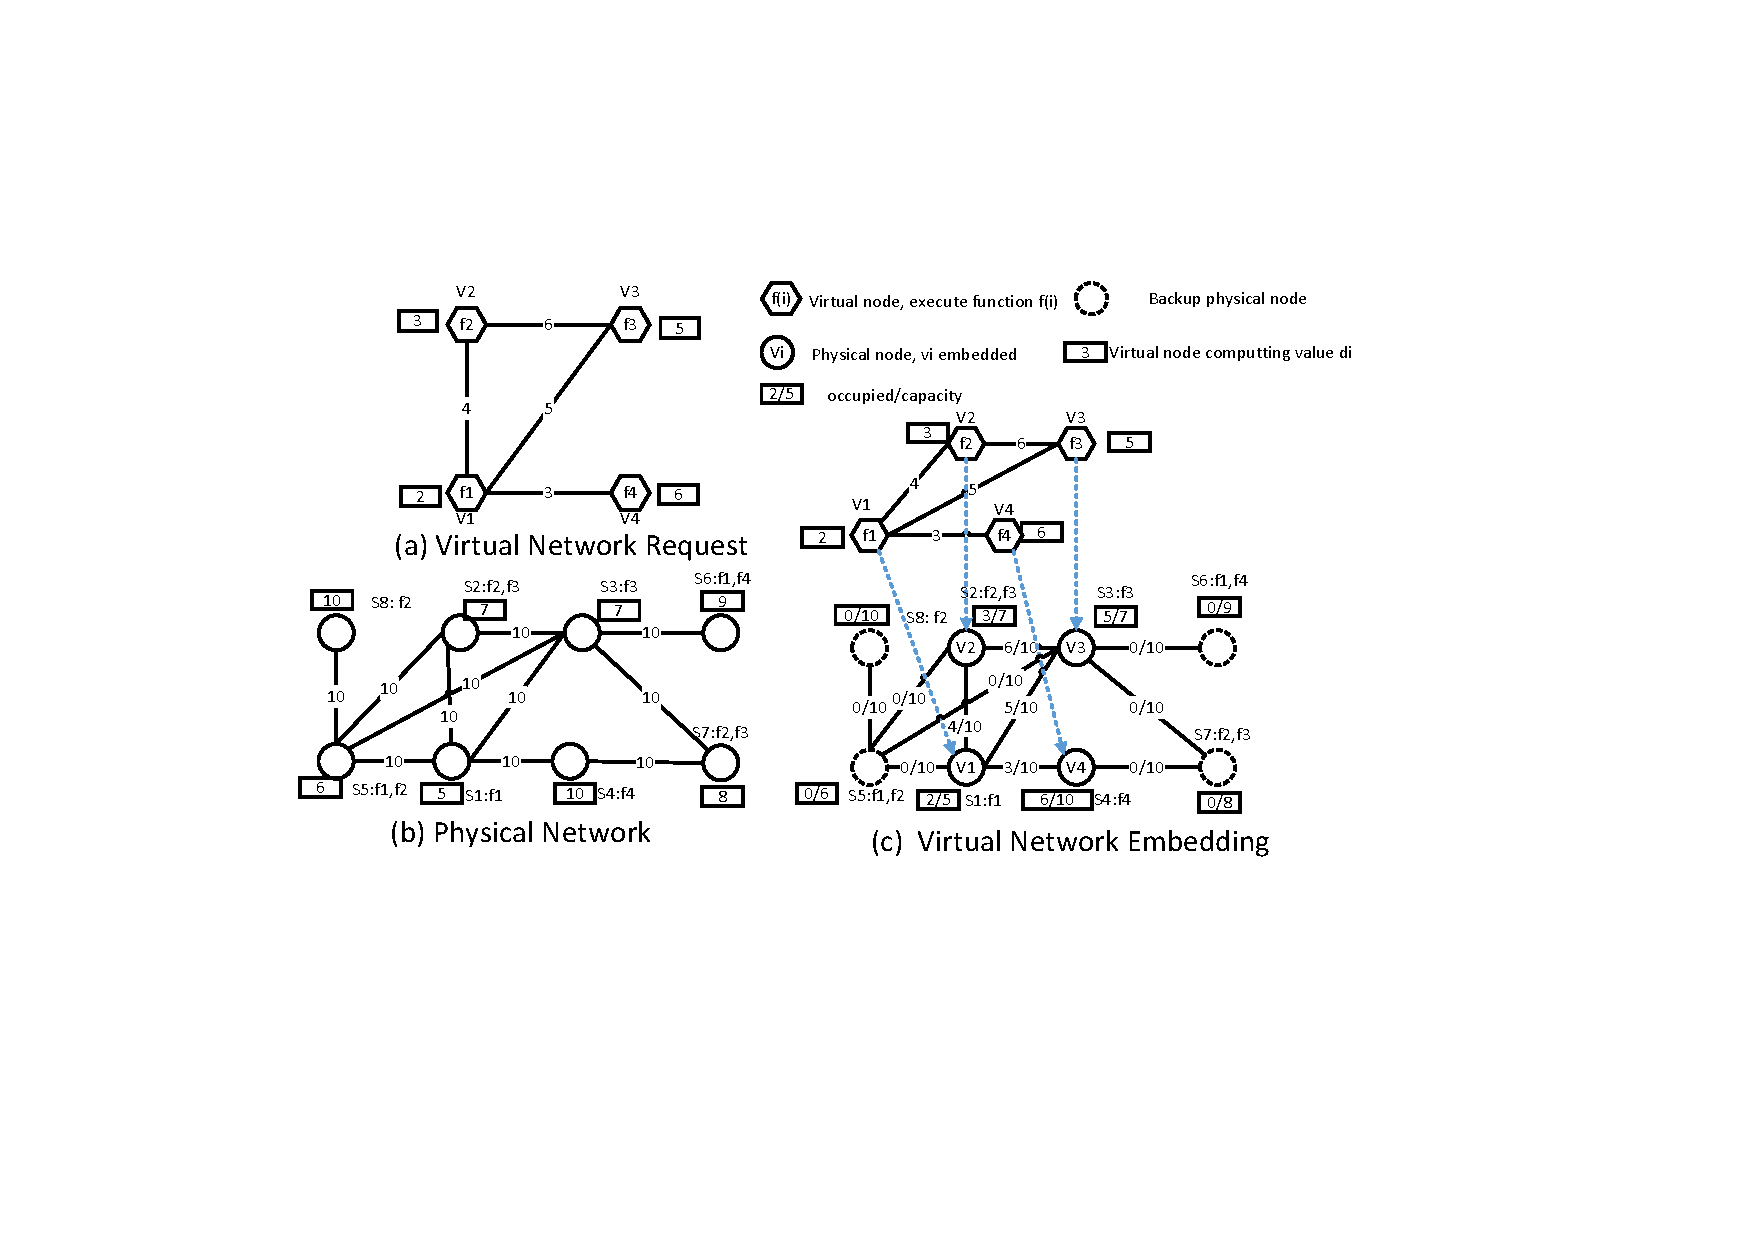
\includegraphics[width=5in]{Fig/VNQSNVNE}\\
\caption{An example of virtual network embedding. (a) Virtual Network Request $G(V,E)$, $V=\{v_1,v_2,v_3,v_4\}$, $E=\{e_{12},e_{23},e_{13},e_{14}\}$,  $f(i)=\{f_1,f_2,f_3,f_4\}$, $d_i=\{2,3,5,6\}$, $d_{ij}=\{4,5,3,6\}. $(b) Physical Network $G(S,L), S=\{s_1,s_2,s_3,s_4,s_5,s_6,s_7,s_8\}, L=\{l_{12},l_{13},l_{14},l_{15},l_{23},l_{25},l_{35},l_{36},l_{37},l_{47},l_{58}\}, F(i)=\{\{f_1\},\{f_2,f_3\},\{f_3\},\{f_4\},\{f_1,f_2\},\{f_1,f_4\},\{f_2,f_3\},\{f_2\}\}, c_i=\{5,7,7,10,6,9,8,10\}, b_{ij}=\{10,10,10,10,10,10,10,10,10,10,10\}$ (c) Vertex mapping $\phi (v_1)=s_1, \phi(v_2)=s_2, \phi (v_3)=s_3, \phi (v_4)=s_4$, link mapping $\rho(e_{12}) = p_{\phi({v_1}) \phi({v_2})}=\{l_{12}\},\rho(e_{23}) = p_{\phi({v_2}) \phi({v_3})}=\{l_{23}\},\rho(e_{13}) = p_{\phi({v_1}) \phi({v_3})}=\{l_{13}\},\rho(e_{14}) = p_{\phi({v_1}) \phi({v_4})}=\{l_{14}\}$.}\label{fig:VNQSNVNE}
\end{figure*}


We model the \textbf{physical network (PN)} as an undirected graph $G (S,L)$, where $S$ and $L$ are the sets of physical nodes and physical links, respectively.
  We use $F(i)$ and $c_i$ to respectively denote the set of feasible virtual functions \rev{that} can be executed on \rev{the physical node  $s_i$ and its} available computational capacity. Each physical link $l_{ij}$ has an available bandwidth of $b_{ij}$. In  the physical network in Fig.\ref{fig:VNQSNVNE}(b) \rev{with the} physical node set $S=\{s_1,s_2,s_3,s_4,s_5,s_6,s_7,s_8\}$ \rev{and}  link set $L=\{l_{12},l_{13},l_{14},l_{15},l_{23},l_{25},l_{35},l_{36},l_{37},l_{47},l_{58}\}$, the  feasible virtual function set of each physical node is  $F(1)=\{f_1\}$, $F(2)=\{f_2,f_3\}$, $F(3)=\{f_3\}$, $F(4)=\{f_4\}$, $F(5)=\{f_1,f_2\}$, $F(6)=\{f_1,f_4\}$, $F(7)=\{f_2,f_3\}$,$F(8)=\{f_2\}$, respectively.



Given \rev{a} VN request $G (V,E)$, the problem of \textbf{\emph{virtual network embedding}} aims to map this request onto the physical network $G (S,L)$ \rev{by} providing enough \rev{resources} as demanded. A feasible mapping should satisfy three constraints, including node capacity constraint, link bandwidth constraint, and function type constraint.

For a virtual node $v_i$, a physical node $s_j$ can hold this virtual node only when both the node capacity constraint  and  the function type constraint  are satisfied. That is, \rev{the capacity request should be satisfied by the physical node with $d_i\leq c_j$, and the required virtual function can be executed on the physical node $s_j$ with ${f_i} \in {F_j}$.} If a physical node $s_j$ satisfies both two  constraints, the node mapping is feasible, and we denote such mapping as $\phi ({v_i}) = {s_j}$.

%Denote the corresponding physical node that holds $v_i$ as $s_j$. Under node capacity constraint, we have $d_i\leq c_j$, that is, the node capacity request should be satisfied by the physical node. Besides capacity constraint, there is a location constraint should be satisfied on the physical node, that is, a virtual node ${v_i} \in V$ can only be provisioned on a physical node $s_j$ with ${f_i} \in {F_j}$. That is, the virtual function running on virtual node ${v_i}$ can be executed on physical node $s_j$. If a physical node $s_j$ satisfies both node capacity constraint and location constraint, the node mapping is feasible, and we denote such mapping as $\phi ({v_i}) = {s_j}$.

For a virtual link $e_{ij}$ \rev{whose two virtual nodes mapped to} physical nodes $s_{i'}$ and $s_{j'}$ (i.e., $\phi({v_i}) = {s_{i'}}$ and $\phi({v_j}) = {s_{j'}}$), \rev{if the link bandwidth constraint is met with $d_{ij}\leq b_{i'j'}$ where $b_{i'j'}$ is the  available bandwidth  of the path connecting nodes $s_{i'}$ and $s_{j'}$, the} virtual link  $e_{ij}$ can be mapped to the physical path $p_{\phi({v_i}) \phi({v_j})}$. We denote the feasible link mapping as $\rho(e_{ij}) = p_{\phi({v_i}) \phi({v_j})}$.

Obviously, to find a feasible virtual network embedding, we should find two mapping functions $\phi$ and $\rho$ to map all the virtual nodes to physical nodes, and all the virtual links to physical paths.


Fig.\ref{fig:VNQSNVNE}(c) shows a feasible virtual network embedding to map the virtual network in Fig.\ref{fig:VNQSNVNE}(a) onto the physical network in Fig.\ref{fig:VNQSNVNE}(b) where  virtual node $v_1$ is embedded in physical node $s_1$, virtual node $v_2$ is embedded in physical node $s_2$, virtual node $v_3$ is embedded in physical node $s_3$, and virtual  node $v_4$ is embedded in physical node $s_4$, respectively. \del{In Fig.\ref{fig:VNQSNVNE}(c),} We also show the resource occupied and available in the physical network after such \rev{a} mapping. For example, for physical node $s_1$, its occupied computation capacity is 2 and the available capacity is 5. %The virtual link $e_{12}$ is mapped to physical link $l_{12}$ , we also draw the occupied bandwidth and the available bandwidth along the physical link  $l_{12}$.
\note{Can multiple virtual nodes be mapped to one physical node? The example only shows one-to-one mapping.}

%, we embed virtual network request as shown in Fig.\ref{fig:VNQSNVNE}(A) into the substrate network, node $v_1$ is embedded in node $s_1$, node $v_2$ is embedded in node $s_2$, node $v_3$ is embedded in node $s_3$, node $v_4$ is embedded in node $s_4$.  node computing demand of every virtual node is not more than these virtual nodes corresponding substrate node's remain node computing. Every link of virtual network request exist a corresponding path consisted of substrate node and remain bandwidth of all links of corresponding path is more than demand  bandwidth of the virtual network link.


%Given the VN request $G (V,E)$ and the physical network  $G (S,L)$, for a feasible mapping, we  denote the mapping physical graph as $G\left( {\hat S,P} \right)$ where $\hat S$ is the physical node set that hold the virtual nodes with $\hat S = \{ {s_{i'}}:\phi({v_i}) = {s_{i'}},for\ {\rm{ }}all\ {v_i} \in V,{s_{i'}} \in S\}$  and $P$ is the path set in which each holds one virtual link with $P = \{ p_{\phi({v_i}) \phi({v_j})}:\rho(e_{ij}) = p_{\phi({v_i}) \phi({v_j})}{\rm{ }}, for\ all,{e_{ij}} \in E\}$. As each virtual link corresponds a physical network path which consisting of multiple physical links, we also denote $G\left( {\hat S,\hat L} \right)$ as the occupying physical network with  $\hat L = \{ {l_{pg}}:{l_{pg}} \in {p_{s_{i'}s_{j'}}}, \rho(e_{ij}) = p_{\phi({v_i}) \phi({v_j})},for\ all\ {e_{ij}} \in E,{l_{pg}} \in L\}$.

 %only subset of $S$ and $L$ are involved to hold the virtual network. We denote the sub-graph as $G\left( {\hat S,\hat L} \right)$ where $\hat S$ is the subset of $S$ and $\hat L$ is the subset of $L$. Obviously, we have $\hat S = \{ {s_{i'}}:{v_i} \to {s_{i'}}{\rm{ }}for{\rm{ }}all{\rm{ }}{v_i} \in V,{s_{i'}} \in S\}$ and $\hat L = \{ {l_{pg}}:{l_{pg}} \in {p_{i'j'}},{e_{ij}} \to {p_{i'j'}}{\rm{ }}for{\rm{ }}all{\rm{ }}{e_{ij}} \in E,{l_{pg}} \in L\}$. We denote $G\left( {\hat S,\hat L} \right)$ as the occupying physical network of the virtual request. As ${e_{ij}} \to {p_{i'j'}}$, that is, each virtual link corresponding a path, we can also denote the mapping physical graph as $G\left( {\hat S,P} \right)$  where $P$ is the corresponding path sets in the process of the embedding mapping.




\rev{A lot of studies have been made to} investigate the virtual network embedding problem \cite{fischer2013virtual}. As the focus of this paper is not \rev{on} virtual network embedding, we adopt \rev{the scheme} in \cite{liu2011completing} as the basic virtual network embedding algorithm. \note{Why did you choose an algorithm from such a poor conference? Or this one is a popular one?}
%There has existed most studies about virtual network embedding method listed in a survey paper\cite{fischer2013virtual}.


\subsection{Survivable virtual network embedding}
Due to malicious attacks, natural disasters, unintentional cable cuts, planned maintenance, equipment malfunctioning, physical nodes that host the virtual nodes may suffer \rev{from unavoidable failure. Failure in the VN can happen when a} single or multiple physical network components fail, which results in financial losses.


In this paper, we first present the problem and the solution of  the survivable virtual network embedding  with single node failure. In section \ref{sec:Extend to multiple physical nodes' failure}, we will discuss how our algorithm can be extended to the scenario with multiple node \rev{failures.}


In the network scenario of \rev{a} single node failure, for a VN request $G (V,E)$ and and its mapping on a physical network $G (S,L)$,  \rev{we aim to add the} minimum backup physical resources to  provide survivable network \rev{services} when any one physical node fails.

\begin{figure}
\centering
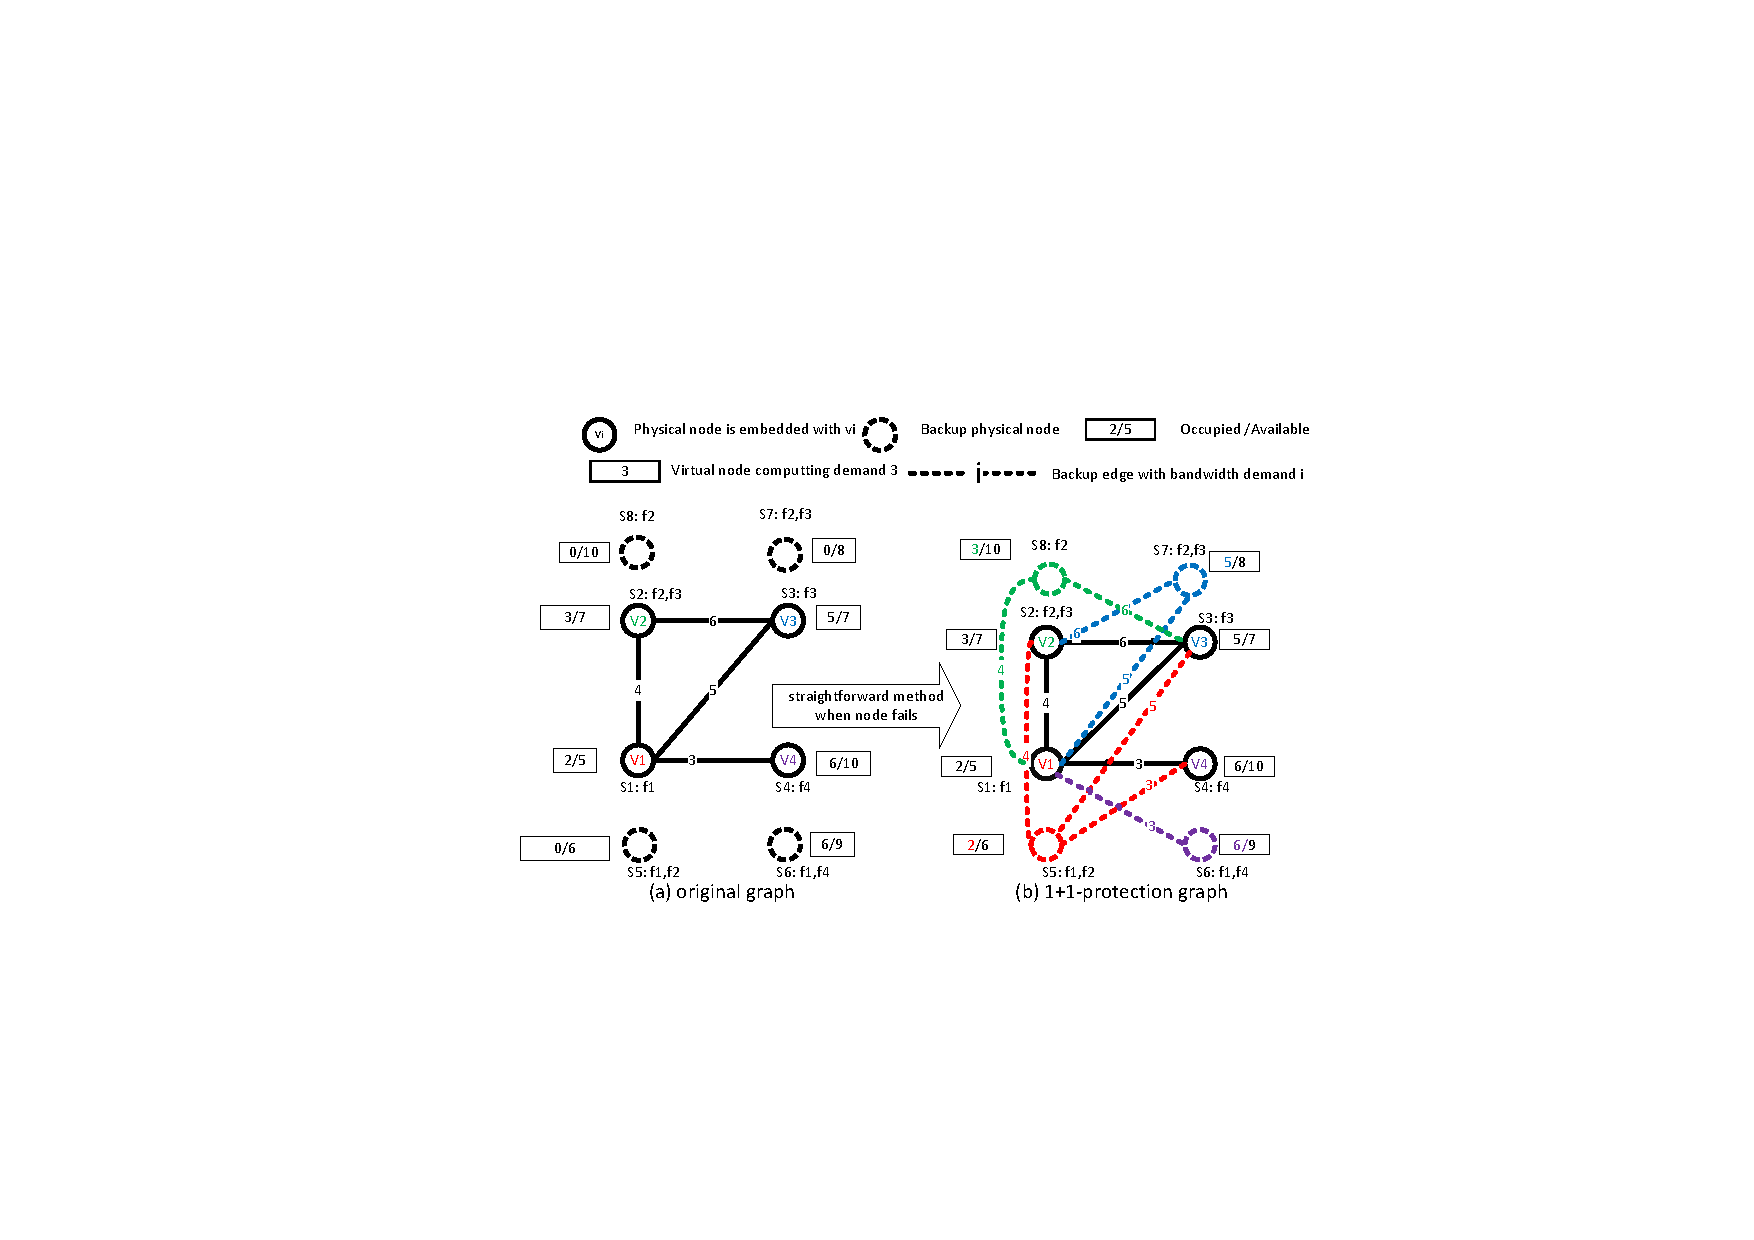
\includegraphics[width=3.5in]{Fig/One2OneProtection}\\
\caption{1+1-protection method}\label{fig:One2OneProtection}
\end{figure}

Node failures not only affect the visualized services running on the failed physical node, but also would terminate all communications which traverse through this node. The \rev{failure of} physical node $ {s_i} \in S $ results in \rev{the disconnection} of physical links in ${L_i} = \left\{ {{l_{ik}}:k \in N(i)} \right\}$  where ${N(i)}$ is the neighbor nodes of node $ {s_i} $.

As we can not predict which node will fail, to handle \rev{a} single node failure, \rev{a straightforward way  is to apply the 1 + 1-protection scheme to set aside the} dedicated backup resource for each virtual node \rev{corresponding to} a VN request.  \rev{In the example of Fig.\ref{fig:One2OneProtection}, a virtual network with  4 virtual nodes are mapped to  4 physical nodes in a physical network.} To provide 1 + 1-protection scheme,  4 backup nodes, 8 backup links are added in the graph.

Although 1 + 1-protection scheme is simple to implement, it requires large amount of  backup resource. The aim of this paper is to provide \rev{the survival network service with the} minimum backup resource cost.


%For example, when node $s_2$ fails, as it runs function $f_2$ for $v_2$ in the VN network, 1 backup node $s_8$ with $F(8)=\{f_2\}$ and 2 backup links $(s_8, s_1)$ and $(s_8, s_3)$ are added. \textbf{For other example, when node $s_1$ fails, as it runs function $f_1$ for $v_1$ in the VN network, one backup node $s_5$ with $F(5)=\{f_1,f_2\}$ and 3 backup links $(s_5, s_2)$,$(s_5, s_3)$ and $(s_5, s_4)$ are added.}.


%, some backup physical node and path should be added. We denote the backup physical node set and link set as $S_b$ and $L_b$.
%
%
%
%
%Survivable virtual network embedding should add  backup resources to guarantee that when a physical node $ {s_i} \in S $ fails, the remaining physical resource plus the backup resources (i.e., $G\left( {\hat S + {S_b} - \{ {s_i}\} ,\hat L + {L_b} - {L_i}} \right)$) can still support a feasible mapping.
%
%
%
%Therefore,  this paper wants to solve the survivable virtual network embedding problem by minimizing the additional resources needed when single node fails. Specially, given virtual network request $G(V,E)$ and its mapping on the physical network $G\left( {\hat S,\hat L} \right)$, add node  and link in the physical network with minimum cost so that when single node fails, the virtual network request $G(V,E)$ can be still satisfied. 